% RP^2 as a circle with half the circumference identified with the other half.
% Source: book/tex/topology/constructions.tex (§ Real projective space).
\documentclass[border=2mm]{standalone}
\usepackage{tikz}
\usepackage{amssymb}
\begin{document}
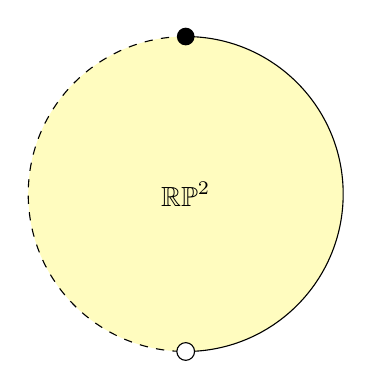
\begin{tikzpicture}[scale=2]
  \fill[yellow!25] (0,0) circle (1);
  \draw (-90:1) arc (-90:90:1);              % right half solid
  \draw[dashed] (90:1) arc (90:270:1);       % left half dashed
  \fill (0,1) circle (1.6pt);
  \draw[fill=white] (0,-1) circle (1.6pt);
  \node at (0,0) {$\mathbb{RP}^2$};
\end{tikzpicture}
\end{document}
